\documentclass[final,hyperref={pdfpagelabels=false}]{beamer}

\usepackage[orientation=portrait,size=a0,scale=1.4]{beamerposter} 
\usetheme{I6pd2}

\usepackage{tikz}
\usepackage{xcolor}
\usepackage{caption}
\usepackage{booktabs}
\usepackage{tcolorbox}
\usepackage[english]{babel}
\usepackage[tight,footnotesize]{subfigure}
\usepackage{amsmath,amsthm,amssymb,latexsym}

\graphicspath{{Images/}}
\usetikzlibrary{bayesnet}
\definecolor{Blue}{HTML}{000080}

\usecaptiontemplate{\small\structure{\insertcaptionname~\insertcaptionnumber: }\insertcaption}

\title{Gaussian Process Latent Space Policies for \\ Data-efficient Learning of Robotic Clothing Assistance\vspace{0.4em}}
\author{Nishanth Koganti$^1$, Tomohiro Shibata$^2$, Tomoya Tamei$^{3}$, and Kazushi Ikeda$^1$} 
\institute{$^1$Nara Institute of Science and Technology, Japan, \\ $^2$Kyushu Institute of Technology, Japan, $^3$Kobe University, Japan}

\newcommand{\leftfoot}{IROS 2018 (Madrid, Spain)}
\newcommand{\rightfoot}{Late Breaking Results}

\begin{document}

\addtobeamertemplate{block end}{}{\vspace*{0.5ex}}
\addtobeamertemplate{block alerted end}{}{\vspace*{2ex}}

\begin{frame}[t]

    \begin{columns}[t]
        \begin{column}{0.02\linewidth}\end{column}

        \begin{column}{0.47\linewidth}
            \begin{block}{Introduction}
                \begin{center}
                    \textbf{Objective}: In this study, we propose the use of Bayesian Gaussian Process Latent Variable Model (BGPLVM)~\cite{bgplvm} to learn a low-dimensional representation of motor-skills. We implement our framework in a practical setting with a dual-arm robot performing clothing assistance tasks.
                \end{center}

                \begin{columns}[t]
                    \begin{column}{0.6\textwidth}
                        ~\\~\\
                        Tamei et al.~\cite{tamei2011} developed clothing assistance robot to perform T-shirt clothing task:

                        \vspace*{1cm}
                        \begin{itemize}
                            \item \textbf{Reinforcement Learning} scheme used to acquire motor skills for cloth handling.\\~\\
                            \item \textbf{Via-points} used as policy representation with one via-point as a policy parameter for fast learning.
                        \end{itemize}
                    \end{column}

                    \begin{column}{0.4\textwidth}
                        \begin{figure}
                            \centering
                            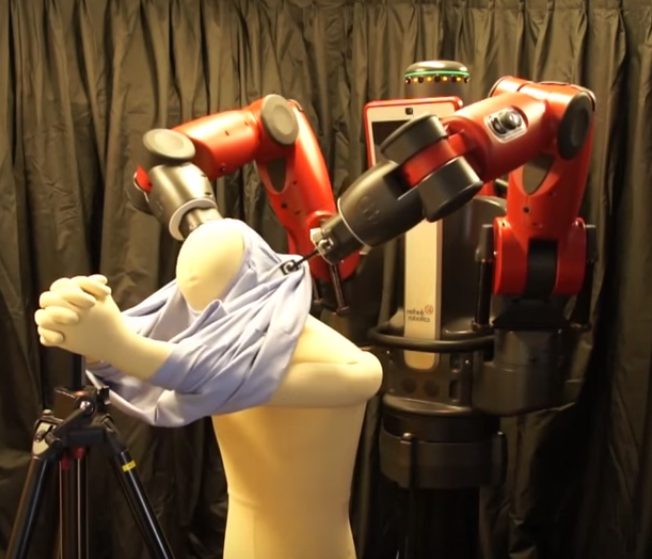
\includegraphics[width=\textwidth]{setup}
                        \end{figure}
                    \end{column}
                \end{columns}
            \end{block}
        \end{column}

        \begin{column}{0.02\linewidth}\end{column}

        \begin{column}{0.47\linewidth}
            \begin{block}{Problem Description}
                \centering Recent focus has been on LVMs for sample-efficient RL~\cite{lrl1, lrl2}.

                \begin{columns}[t]
                    \begin{column}{0.8\textwidth}
                        \begin{itemize}
                            \setlength{\itemindent}{1in}
                            \item Latent variable model (Titsias et al., 2010~\cite{bgplvm}):
                            \begin{equation*}
                                \mathbf{y} = f(\mathbf{x}) + \epsilon, \epsilon \sim \mathcal{N}(\mathbf{0}, \sigma^2 \mathbf{I})
                            \end{equation*}
                            \item $f: \mathbf{x} \rightarrow \mathbf{y}$: Mapping given by a Gaussian process. \vspace*{1em}
                            \item Automatic dimensionality reduction perfomed using ARD kernel:
                            \begin{equation*}
                                \displaystyle
                                k(x, x') = \sigma_f^2 \exp \left( -\frac{1}{2} \sum_{q=1}^Q \textcolor{blue}{w_q} (x_q - x_q')^2 \right)
                            \end{equation*}
                            \vspace*{0.5em}
                        \end{itemize} 
                    \end{column}

                    \begin{column}{0.2\textwidth}
                        \begin{figure}[t]
                            \centering
                            \vspace*{0.5cm}
                            \scalebox{1.5}{
                                \tikz{%
                                    \node[latent] (x) {$\mathbf{x}$};
                                    \node[latent, right=of x] (f) {$f$};
                                    \node[const, above=of f] (w) {$\Phi$};
                                    \node[obs, below=of x] (y) {$\mathbf{y}$};
                                    \edge {x} {y};
                                    \edge {f} {y};
                                    \edge {w} {f};
                                \edge {w} {x};
                                    }
                            }
                        \end{figure}
                    \end{column}
                \end{columns}

                \begin{columns}
                    \begin{column}{0.7\textwidth}
                        \begin{figure}
                            \centering
                            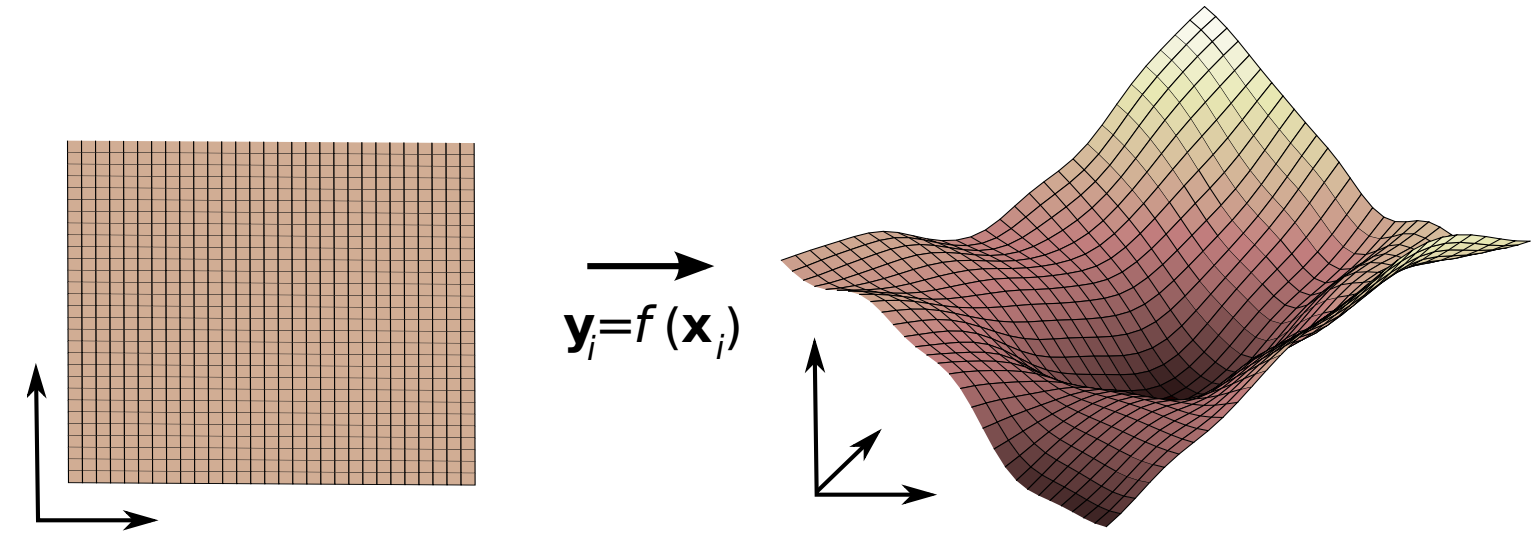
\includegraphics[width=0.8\textwidth]{nonlinearMap}
                        \end{figure}
                    \end{column}

                    \begin{column}{0.3\textwidth}
                        \begin{figure}
                            \centering
                            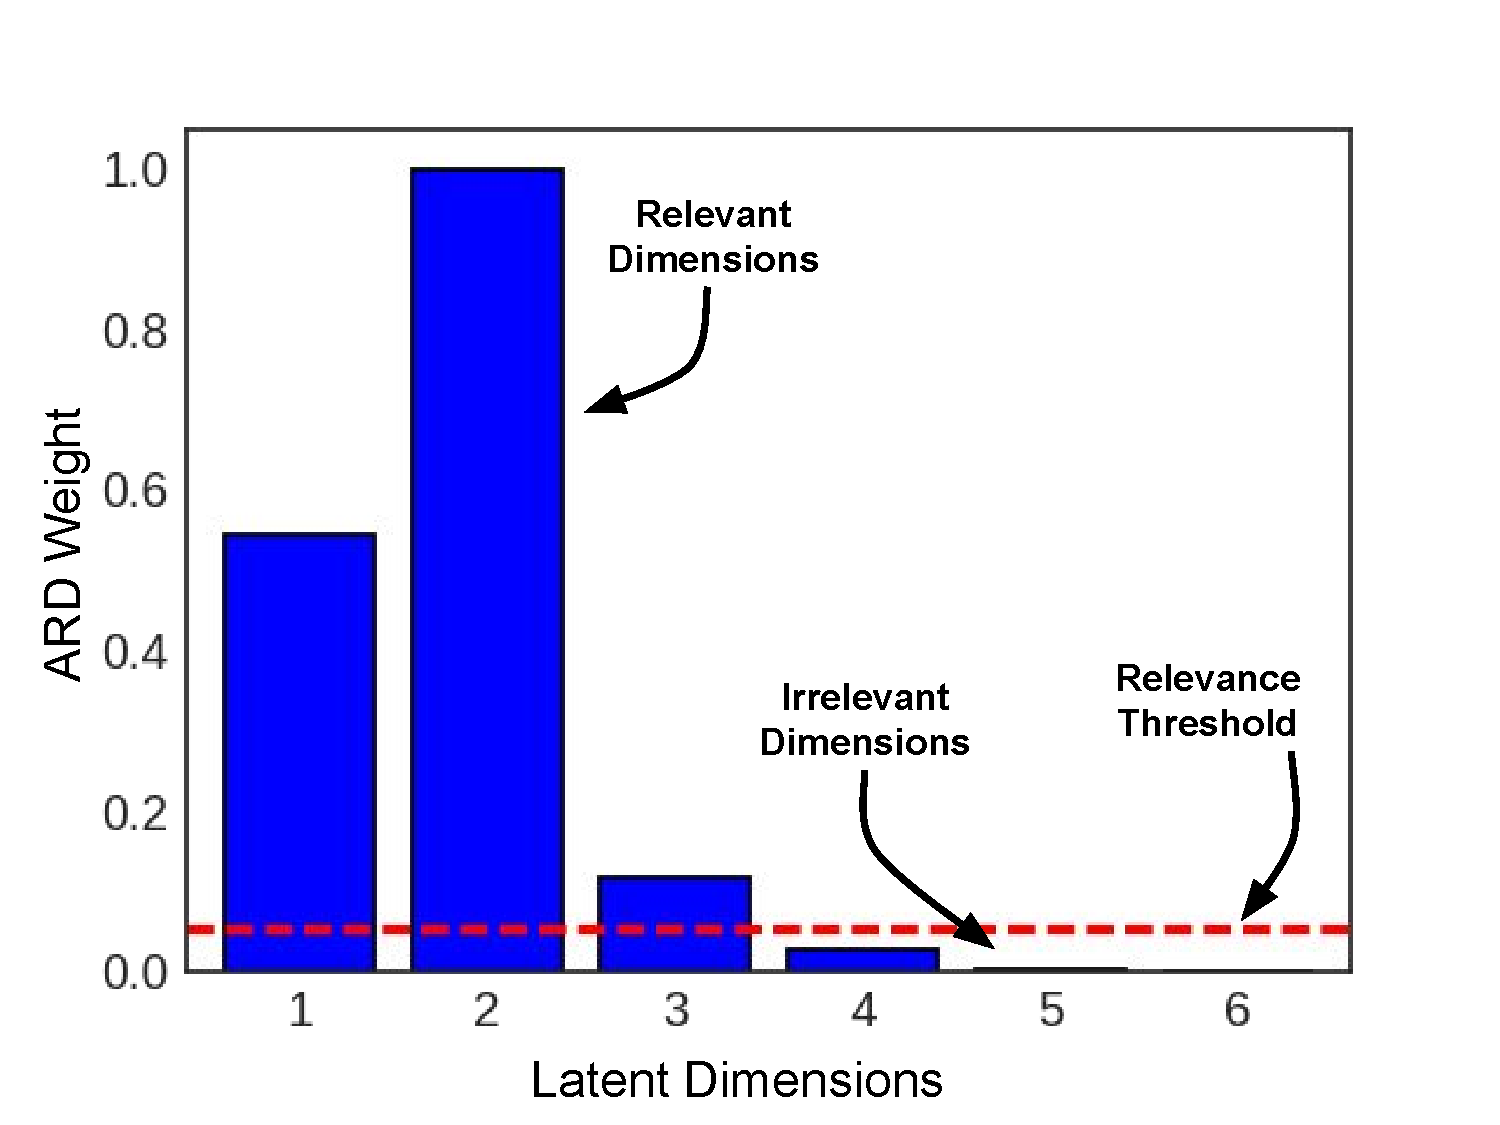
\includegraphics[width=\textwidth]{ard}
                        \end{figure}
                    \end{column}
                \end{columns}
            \end{block}
        \end{column}

        \begin{column}{0.02\linewidth}\end{column}
    \end{columns}

    \begin{columns}[t]
        \begin{column}{0.02\linewidth}\end{column}

        \begin{column}{0.96\linewidth}
            \begin{alertblock}{Proposed Method}
                \begin{columns}[t]
                    \begin{column}{0.3\textwidth}
                        \centering \textbf{Interface for Latent Space Control}

                        \begin{itemize}
                            \item Inexperienced users can impart noisy demonstrations. \vspace*{0.5em}
                            \item User-friendly interface: Cursor control in latent space. \vspace*{1em}
                        \end{itemize}

                        \begin{figure}
                            \centering
                            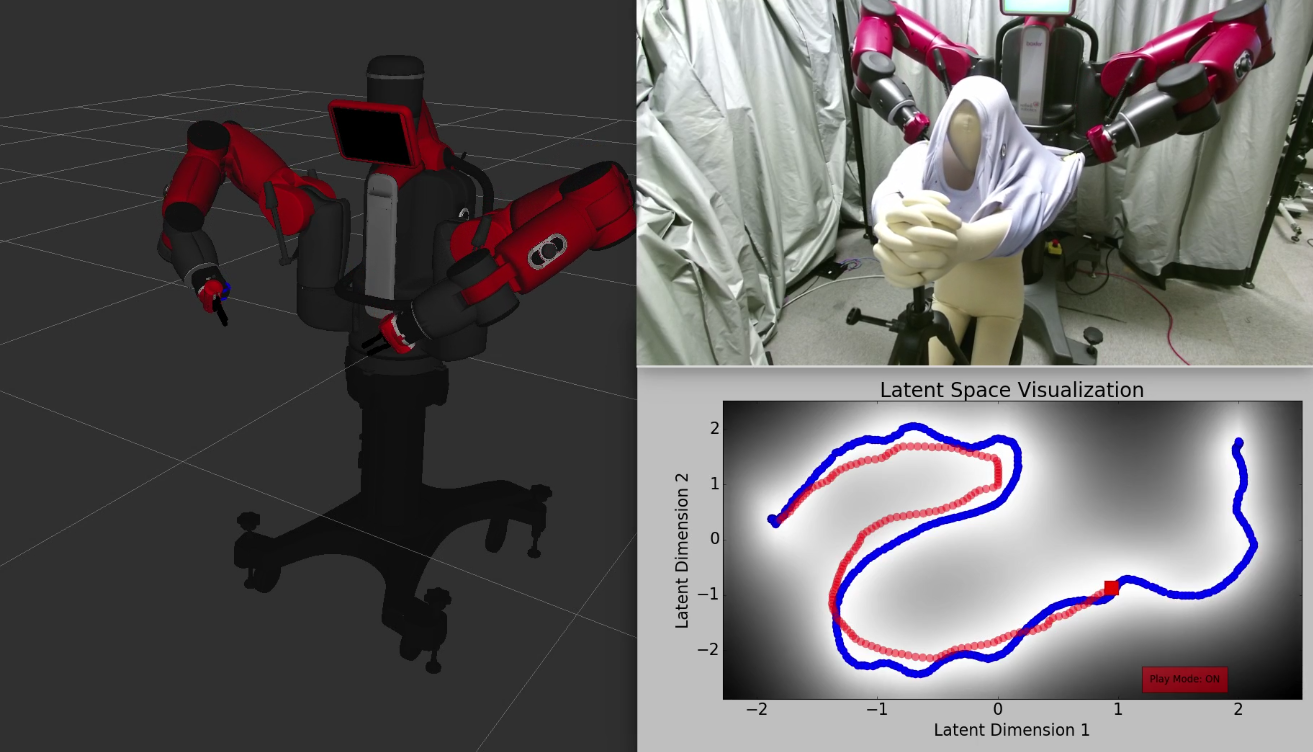
\includegraphics[width=0.8\textwidth]{controller}
                            \vspace*{1em}
                            \caption*{\centering User-interface for latent space controller. 2D latent space sufficient to control high DoF dual-arm robot.}
                        \end{figure}
                    \end{column}

                    \begin{column}{0.4\textwidth}
                        \centering \textbf{Method Overview}

                        \begin{figure}
                            \centering
                            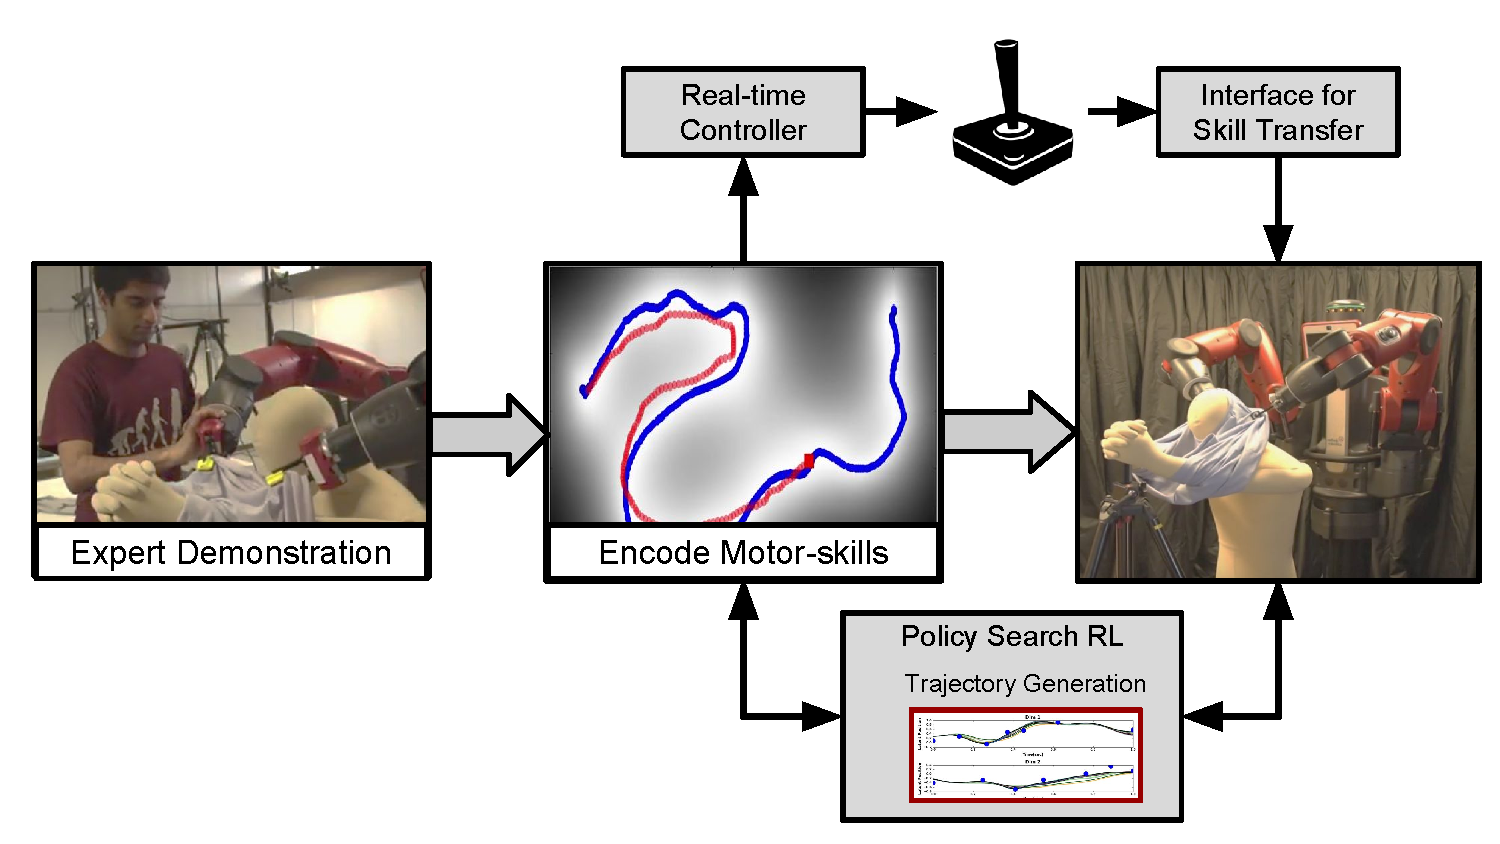
\includegraphics[width=\textwidth]{overview}
                        \end{figure}
                    \end{column}

                    \begin{column}{0.3\textwidth}
                        \centering \textbf{Latent Space Policy Search}

                        \centering Data-efficient Learning: Perform policy search in low-dimensional BGPLVM space. 

                        \begin{itemize}
                            \item Policy Search: PoWER algorithm, Representation: Dynamic movement primitives.
                        \end{itemize}

                        \begin{figure}
                            \centering
                            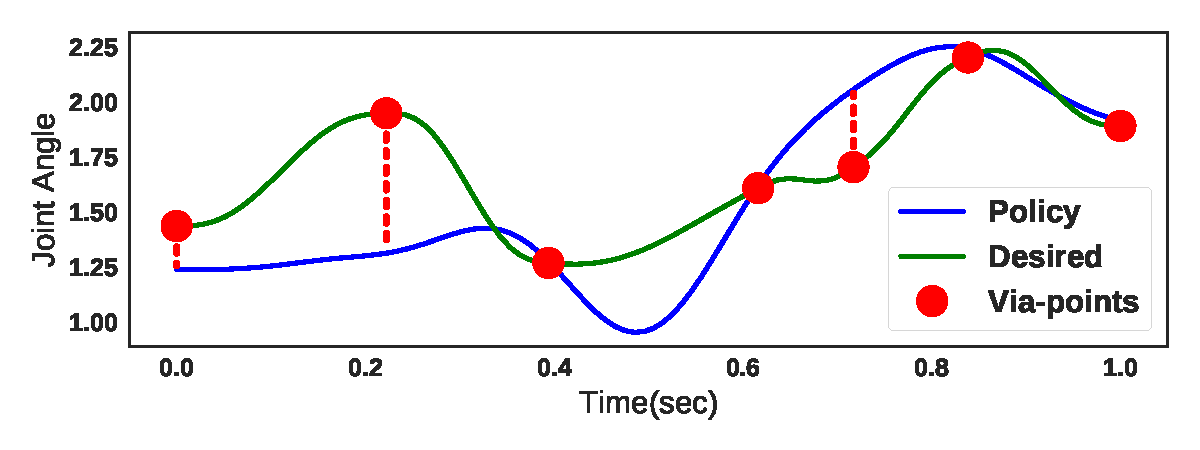
\includegraphics[width=\textwidth]{rewards}
                        \end{figure}

                        \begin{itemize}
                            \item Represent reward function by distance from desired Via-points to current policy:
                            \begin{equation*}
                                R(\pi(\theta)) = \sum_{i=1}^{n_{\text{dims}}} \sum_{j=1}^{n_{\text{via}}} \| V_{i,j} - \pi_i(\theta, t_{i,j}) \|^2
                            \end{equation*}
                        \end{itemize}
                    \end{column}
                \end{columns}
            \end{alertblock}
            \vspace*{2cm}
            \begin{alertblock}{Experimental Results}
                \begin{columns}[t]
                    \begin{column}{0.33\textwidth}
                        \centering \textbf{Comparison of Latent Variable Models}

                        \begin{itemize}
                            \item \textbf{Evaluation}: Reconstruction error of LVM with NRMSE.
                            \item \textbf{Dataset}: Demonstration of clothing assistance by 3 subjects for 6 postures of mannequin.
                        \end{itemize}
                        \vspace*{1cm}
                        \begin{figure}
                            \centering
                            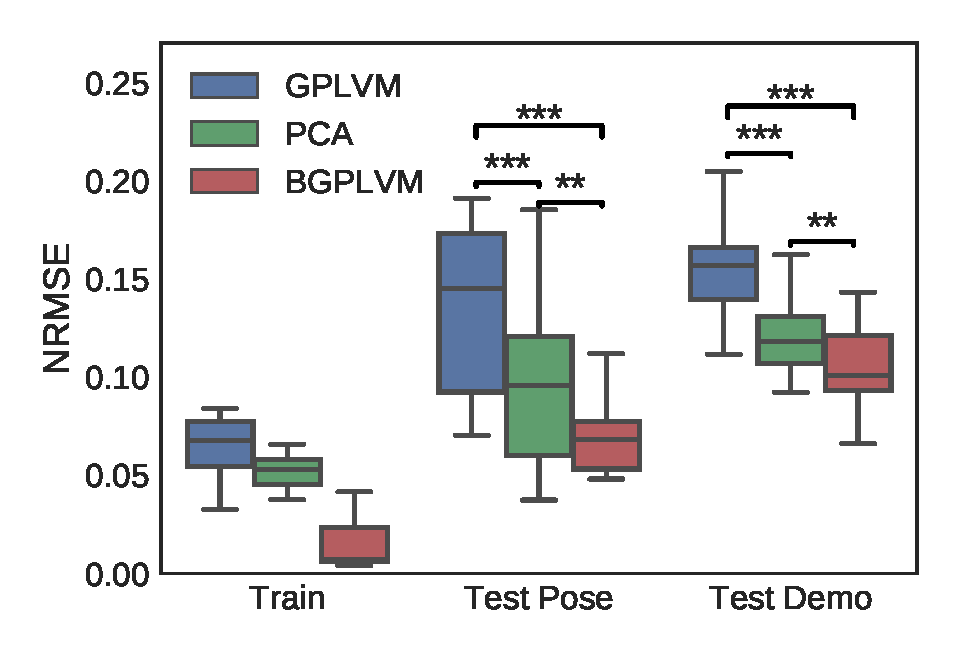
\includegraphics[width=\textwidth]{jaError}
                        \end{figure}
                    \end{column}

                    \begin{column}{0.33\textwidth}
                        \centering \textbf{Trajectory Generation using Controller}
                        \begin{itemize}
                            \item \textbf{Evaluation}: 5 subjects used controller to impart skills.
                        \end{itemize}
                        \begin{figure}
                            \centering
                            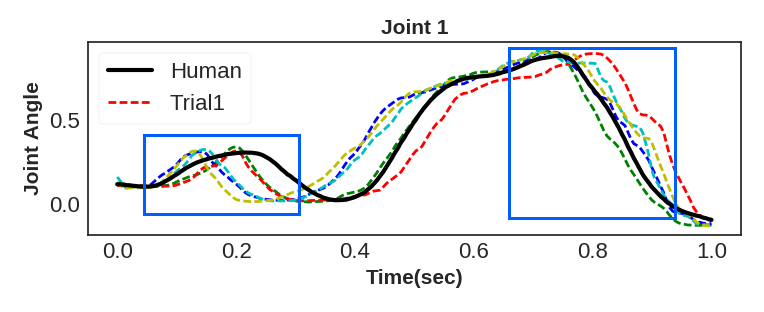
\includegraphics[width=\textwidth]{controllerVar}
                        \end{figure}
                        \vspace*{-1cm}
                        \begin{figure}
                            \centering
                            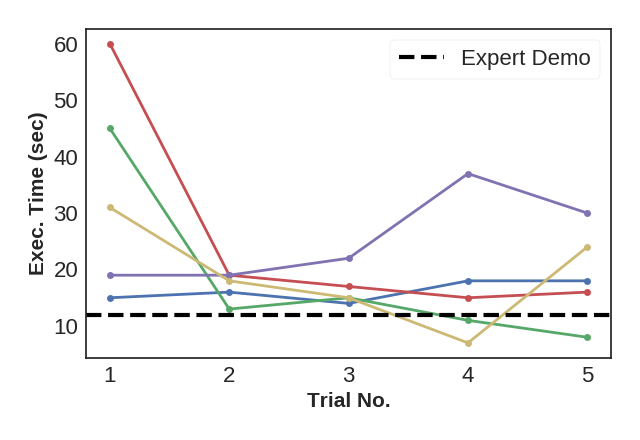
\includegraphics[width=\textwidth, height=0.15\textheight]{controllerTime}
                        \end{figure}
                    \end{column}

                    \begin{column}{0.33\textwidth}
                        \centering \textbf{Evaluation of Latent Space Policy Search}

                        \begin{itemize}
                            \item Apply RL in different latent spaces with same formuation. \vspace*{0.5cm}
                            \item Parameters: $50 \times n_{\text{dims}}$ basis functions. \vspace*{0.5cm}
                            \item PoWER: 10 best iterations used for parameter updates.
                        \end{itemize}
                        \vspace*{1cm}
                        \begin{figure}
                            \centering
                            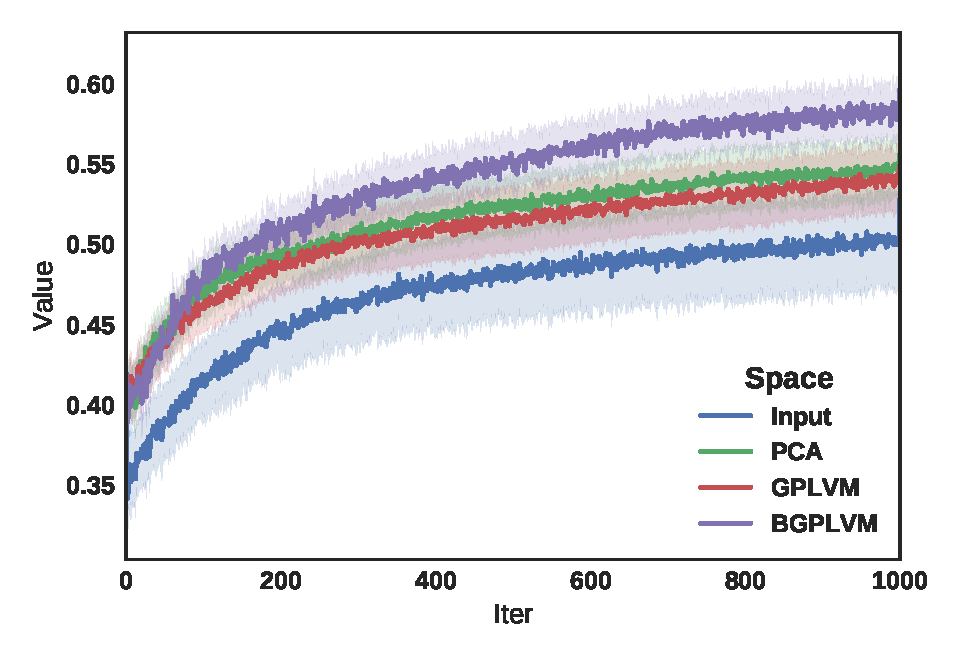
\includegraphics[width=\textwidth]{rlCurves}
                        \end{figure}
                    \end{column}
                \end{columns}
            \end{alertblock}
        \end{column}

        \begin{column}{0.02\textwidth}\end{column}
    \end{columns}

    \begin{columns}[t]
        \begin{column}{.02\textwidth}\end{column}

        \begin{column}{0.47\textwidth}
            \begin{block}{Discussion and Future Work}
                \begin{itemize}
                    \item BGPLVM can encode motor-skills for clothing assistance. \vspace*{1cm}
                    \item Future Work: Learn from human preferences using latent space controller. \vspace*{1cm}
                    \item Combine dimensionality reduction with policy search.
                \end{itemize}
            \end{block}
        \end{column}

        \begin{column}{0.47\textwidth}
            \begin{block}{References}
                \nocite{*}
                \scriptsize{
                    \bibliographystyle{unsrt}
                    \begin{thebibliography}{10}
                        \bibitem{bgplvm}
                        Titsias, Michalis, and Neil D. Lawrence. ``Bayesian Gaussian process latent variable model.'' Proceedings of the Thirteenth International Conference on Artificial Intelligence and Statistics. AISTATS 2010.
                        \bibitem{tamei2011}
                        Tamei, Tomoya, et al. ``Reinforcement learning of clothing assistance with a dual-arm robot.'' Humanoid Robots (Humanoids), 2011 11th IEEE-RAS International Conference on. IEEE, 2011.
                        \bibitem{lrl1}
                        Sæmundsson, Steindór, et al. ``Meta Reinforcement Learning with Latent Variable Gaussian Processes.'' arXiv preprint arXiv:1803.07551 (2018).
                        \bibitem{lrl2}
                        Haarnoja, Tuomas, et al. ``Latent Space Policies for Hierarchical Reinforcement Learning.'' arXiv preprint arXiv:1804.02808 (2018).
                    \end{thebibliography}}
            \end{block}
        \end{column}

        \begin{column}{.02\textwidth}\end{column}
    \end{columns}

\end{frame}

\end{document}
